\section{Runge--Kutta方法}
\label{sec:odenum-runge-kutta}

Euler方法整步只用起点的斜率，弯曲的解曲线被它的切线代替。要想更准，自然想到在这一步内部多看几次斜率，再把它们组合起来。看哪几处、怎样组合，才能真正提高阶数？

\paragraph{主要思想：匹配Taylor展开}
先看真解一步走到哪里。设$\bm{f}$二次连续可微，记
\begin{equation}
 \bm{g}=\partial_t\bm{f}+\partial_{\bm{x}}\bm{f}\,\bm{f},
 \label{eq:odenum-total-derivative}
\end{equation}
它是$\bm{f}$沿解的全导数，也就是$\ddot{\bm{x}}$。解的Taylor展开为
\[
 \bm{x}(t+h)=\bm{x}+h\bm{f}+\frac{h^2}{2}\bm{g}+O(h^3),
\]
右端各量在$(t,\bm{x}(t))$处取值。Euler方法只匹配了前两项，$h^2$一项就是它的局部误差。

现在允许多读一次斜率。先取起点斜率，再沿它试探着走到$t+\alpha h$，在那里读第二个斜率：
\[
 \bm{k}_1=\bm{f}(t,\bm{x}),\qquad
 \bm{k}_2=\bm{f}\bigl(t+\alpha h,\bm{x}+\alpha h\bm{k}_1\bigr).
\]
最后用两个斜率的加权平均前进：
\[
 \bm{\Psi}_h(t,\bm{x})=\bm{x}+h\bigl(b_1\bm{k}_1+b_2\bm{k}_2\bigr).
\]

$\alpha,b_1,b_2$待定。把$\bm{k}_2$在$(t,\bm{x})$处作Taylor展开，$h$的一次项正好由式~\eqref{eq:odenum-total-derivative}的全导数给出：
\[
 \bm{k}_2=\bm{f}+\alpha h\,\bm{g}+O(h^2).
\]
代入更新式，得到
\[
 \bm{\Psi}_h(t,\bm{x})=\bm{x}+(b_1+b_2)h\bm{f}+\alpha b_2h^2\bm{g}+O(h^3).
\]

与真解的展开逐项比较，要让$h$和$h^2$的系数都对上，需要
\begin{equation}
 b_1+b_2=1,\qquad \alpha b_2=\frac{1}{2}.
 \label{eq:odenum-two-stage-conditions}
\end{equation}
三个未知数、两个方程，于是有一族二阶方法。取$\alpha=1/2$，$b_1=0$，$b_2=1$，得到\term{中点方法}（midpoint method）：
\begin{equation}
 \begin{aligned}
  \bm{k}_1&=\bm{f}\bigl(t_k,\bm{x}^{(k)}\bigr),\\
  \bm{k}_2&=\bm{f}\Bigl(t_k+\frac{h}{2},\ \bm{x}^{(k)}+\frac{h}{2}\bm{k}_1\Bigr),\\
  \bm{x}^{(k+1)}&=\bm{x}^{(k)}+h\bm{k}_2.
 \end{aligned}
 \label{eq:odenum-midpoint}
\end{equation}
另一个选择$\alpha=1$，$b_1=b_2=1/2$是Heun方法，它在第~\ref{sec:odenum-adaptive}节还要用到。

中点方法的几何含义很清楚（图~\ref{fig:odenum-midpoint-steps}）：积分$\int\bm{f}\,\mathrm{d}s$用区间中点的值乘$h$来近似，这是中点求积公式。困难在于中点处的状态未知，于是先用起点斜率走半步来试探它。试探点本身只有一阶精度，但$\bm{f}$在那里的值只需准到$O(h^2)$，一乘$h$就足够了。

\begin{BookInlineFigure}
 \centering
 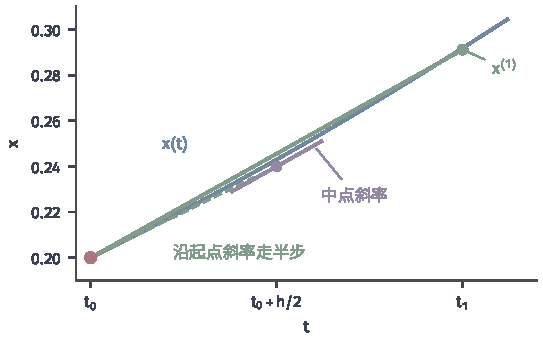
\includegraphics[width=92mm]{figures/06-differential-equations/01-ordinary-differential-equations/matplotlib/odenum-midpoint-steps/figure.pdf}
 \caption{中点方法的第一步，$h=1/2$，问题为式~\eqref{eq:odenum-running}。蓝线是真解，绿色虚线沿起点斜率走半步到紫点，紫色短线是在紫点读到的斜率$k_2$，绿色实线从红色初值出发，沿斜率$k_2$走满一步到$x^{(1)}$。}
 \label{fig:odenum-midpoint-steps}
\end{BookInlineFigure}

中点方法的手算只需把式~\eqref{eq:odenum-midpoint}代入两轮。对例~\eqref{eq:odenum-running}取$h=0.5$，第一轮的结果为
\[
 k_1=0.16,\qquad 0.2+0.25k_1=0.24,\qquad k_2=0.24\times0.76=0.1824,
\]
于是
\[
 x^{(1)}=0.2+0.5\times0.1824=0.2912.
\]
第二轮从$x^{(1)}$出发，同样得到
\[
 k_1=0.206403,\qquad 0.342801,\qquad k_2=0.225288,
\]
所以$x^{(2)}=0.403844$，终点误差约$-7.7\times10^{-4}$，比Euler方法的$-0.0238$小了约三十倍，而右端求值次数只从$2$增加到$4$。

\paragraph{主要思想：多级与经典四阶方法}
上面的做法可以一般化。$s$级\term{显式Runge--Kutta方法}（explicit Runge--Kutta method）依次计算$s$个\term{阶段斜率}（stage slope）：
\begin{equation}
 \bm{k}_i=\bm{f}\Bigl(t_k+c_ih,\ \bm{x}^{(k)}+h\sum_{j<i}a_{i,j}\bm{k}_j\Bigr),\quad i=1,\ldots,s,
 \label{eq:odenum-rk-stages}
\end{equation}
再组合成一步更新：
\begin{equation}
 \bm{x}^{(k+1)}=\bm{x}^{(k)}+h\sum_{i=1}^{s}b_i\bm{k}_i.
 \label{eq:odenum-rk-update}
\end{equation}
每个$\bm{k}_i$只用前面已算出的斜率，所以依次代入即可，这就是“显式”的含义。系数由匹配Taylor展开决定，中点方法是$s=2$的情形。

阶数越高，要匹配的项越多。沿解的高阶全导数含有$\bm{f}$的各阶偏导的多种组合，四阶需要同时满足八个代数条件。最著名的解是\term{经典四阶Runge--Kutta方法}（classical fourth-order Runge--Kutta method），简称RK4：
\begin{equation}
 \begin{aligned}
  \bm{k}_1&=\bm{f}\bigl(t_k,\bm{x}^{(k)}\bigr),\\
  \bm{k}_2&=\bm{f}\Bigl(t_k+\frac{h}{2},\ \bm{x}^{(k)}+\frac{h}{2}\bm{k}_1\Bigr),\\
  \bm{k}_3&=\bm{f}\Bigl(t_k+\frac{h}{2},\ \bm{x}^{(k)}+\frac{h}{2}\bm{k}_2\Bigr),\\
  \bm{k}_4&=\bm{f}\bigl(t_k+h,\ \bm{x}^{(k)}+h\bm{k}_3\bigr),\\
  \bm{x}^{(k+1)}&=\bm{x}^{(k)}+\frac{h}{6}\bigl(\bm{k}_1+2\bm{k}_2+2\bm{k}_3+\bm{k}_4\bigr).
 \end{aligned}
 \label{eq:odenum-rk4}
\end{equation}

权重$1,2,2,1$有一个可以直接验证的来源。若$\bm{f}$不依赖状态，四个斜率分别是$\bm{f}(t_k)$、$\bm{f}(t_k+h/2)$、$\bm{f}(t_k+h/2)$、$\bm{f}(t_k+h)$，更新式化为
\[
 \bm{x}^{(k+1)}-\bm{x}^{(k)}=\frac{h}{6}\Bigl(\bm{f}(t_k)+4\bm{f}\bigl(t_k+\tfrac{h}{2}\bigr)+\bm{f}(t_k+h)\Bigr),
\]
正是Simpson求积公式。中点权重$4$被拆给了两个中点估计$\bm{k}_2$和$\bm{k}_3$，它们从不同的试探点读取斜率，彼此修正。

\begin{theorem}[RK4的阶]
 \label{thm:odenum-rk4-order}
 设$\bm{f}$在包含解曲线的开集上四次连续可微，$\bm{x}(t)$是$[t_0,t_0+T]$上的解。则存在$C,h_0>0$，使当$0<h\leq h_0$时，RK4的局部截断误差满足
 \begin{equation}
  \bigl\lVert\bm{\ell}^{(k+1)}\bigr\rVert_2\leq Ch^{5}.
  \label{eq:odenum-rk4-local}
 \end{equation}
\end{theorem}

这个结论的证明需要把真解和数值更新都展开到$h^4$，逐项核对八个代数条件，篇幅较长，读者可查阅\scite{math-hairer1993ode}。定理的条件不能省：光滑性决定了展开能够进行到第几项，下文的例子会说明它不成立时阶数怎样丢失。

\paragraph{计算过程}
RK4每一步按式~\eqref{eq:odenum-rk4}依次算四个斜率。下面仍用例~\eqref{eq:odenum-running}的数据手算，取$h=0.5$，$N=2$。

\needspace{6\baselineskip}
\paragraph{变量}
\begin{itemize}
 \item $\bm{x}^{(k)}\in\mathbb{R}^{n}$：第$k$个网格点的数值解。
 \item $\bm{k}_1,\bm{k}_2,\bm{k}_3,\bm{k}_4\in\mathbb{R}^{n}$：本步的四个阶段斜率，用完即弃。
 \item $\bm{y}_2,\bm{y}_3,\bm{y}_4\in\mathbb{R}^{n}$：读取后三个斜率的试探状态。
\end{itemize}

\paragraph{初始化}
与Euler方法相同，把数值解初始化为初值。例中
\[
 x^{(0)}=0.2,\qquad t_0=0,\qquad h=0.5,\qquad N=2.
\]

\needspace{6\baselineskip}
\paragraph{每轮更新}
对$k=0,1,\ldots,N-1$依次执行：
\begin{enumerate}

 \item \textbf{起点斜率。}计算$\bm{k}_1=\bm{f}(t_k,\bm{x}^{(k)})$。例中第一轮
 \[
  k_1=0.2\times0.8=0.16.
 \]

 \item \textbf{第一次试探中点。}令
 \[
  \bm{y}_2=\bm{x}^{(k)}+\frac{h}{2}\bm{k}_1,\qquad \bm{k}_2=\bm{f}\bigl(t_k+\tfrac{h}{2},\bm{y}_2\bigr).
 \]
 例中第一轮
 \[
  y_2=0.24,\qquad k_2=0.24\times0.76=0.1824.
 \]

 \item \textbf{第二次试探中点。}令
 \[
  \bm{y}_3=\bm{x}^{(k)}+\frac{h}{2}\bm{k}_2,\qquad \bm{k}_3=\bm{f}\bigl(t_k+\tfrac{h}{2},\bm{y}_3\bigr).
 \]
 例中第一轮
 \[
  y_3=0.2456,\qquad k_3=0.2456\times0.7544=0.185281.
 \]

 \item \textbf{试探终点。}令
 \[
  \bm{y}_4=\bm{x}^{(k)}+h\bm{k}_3,\qquad \bm{k}_4=\bm{f}\bigl(t_k+h,\bm{y}_4\bigr).
 \]
 例中第一轮
 \[
  y_4=0.292640,\qquad k_4=0.207002.
 \]

 \item \textbf{加权前进。}由式~\eqref{eq:odenum-rk4}的最后一行计算$\bm{x}^{(k+1)}$。例中第一轮
 \[
  x^{(1)}=0.2+\frac{0.5}{6}\times1.102363=0.2918636.
 \]
 例中第二轮从$x^{(1)}$出发，依次得到
 \[
  \begin{gathered}
   k_1=0.206679,\quad y_2=0.343533,\quad k_2=0.225518,\\
   y_3=0.348243,\quad k_3=0.226970,\\
   y_4=0.405349,\quad k_4=0.241041,
  \end{gathered}
 \]
 于是
 \[
  x^{(2)}=0.2918636+\frac{0.5}{6}\times1.352696=0.4045883.
 \]

 \item \textbf{停止。}当$k+1=N$时结束。例中$k+1=2$，退出循环。
\end{enumerate}
最终例中得到$x^{(2)}=0.404588$，真值为$0.404610$，误差约$-2.1\times10^{-5}$，只用了$8$次右端求值。图~\ref{fig:odenum-rk4-stages}标出第一步的四个采样位置。

\begin{BookInlineFigure}
 \centering
 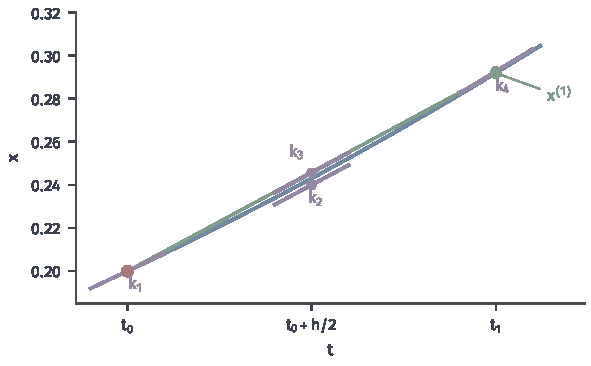
\includegraphics[width=100mm]{figures/06-differential-equations/01-ordinary-differential-equations/matplotlib/odenum-rk4-stages/figure.pdf}
 \caption{RK4的第一步，$h=1/2$，问题为式~\eqref{eq:odenum-running}。紫点是四个采样位置$(t_0,x_0)$、$(t_0+h/2,y_2)$、$(t_0+h/2,y_3)$、$(t_1,y_4)$，紫色短线是读到的四个斜率；绿线从红色初值走到$x^{(1)}$，蓝线是真解。}
 \label{fig:odenum-rk4-stages}
\end{BookInlineFigure}

\paragraph{光滑性决定阶数能否兑现}
定理~\ref{thm:odenum-rk4-order}要求右端足够光滑。把例~\eqref{eq:odenum-running}改成带时间跳变的方程：
\[
 \dot{x}=r(t)x(1-x),\qquad
 r(t)=\begin{cases}1,&t<t_{*},\\2,&t\geq t_{*},\end{cases}
\]
其中$t_{*}=1/\sqrt{2}$，闭式解用$\int_0^tr$代替$t$仍然成立。图~\ref{fig:odenum-rk4-jump}的红线是均匀网格上RK4的终点误差。$t_{*}$落在某一步内部，四个采样点无法判断跳变发生在这一步的什么位置，这一步的局部误差只有$O(h)$，一步就把全局误差拖到一阶，并随$t_{*}$在步内的相对位置起伏。

\begin{BookInlineFigure}
 \centering
 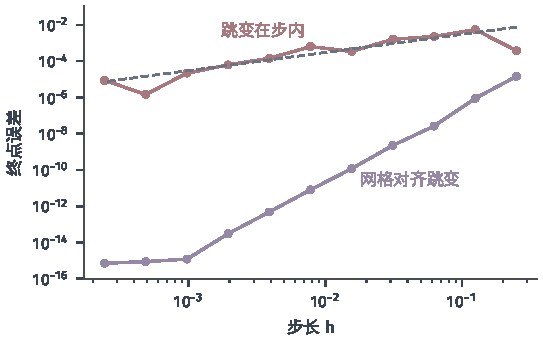
\includegraphics[width=92mm]{figures/06-differential-equations/01-ordinary-differential-equations/matplotlib/odenum-rk4-jump/figure.pdf}
 \caption{右端带跳变时RK4的终点误差。红线：均匀网格，跳变点$t_{*}=1/\sqrt{2}$落在步内；灰色虚线是参考直线$0.03h$。紫线：把$t_{*}$放在网格点上，两侧分别用均匀步长积分，四阶恢复，直到舍入误差使曲线变平。}
 \label{fig:odenum-rk4-jump}
\end{BookInlineFigure}

补救办法也在图中。若已知跳变时刻，把它放到网格点上，在两侧分别积分（紫线），每段内部$\bm{f}$都是光滑的，阶数恢复为四。

\paragraph{每步成本与总成本}
高阶方法每步更贵，比较时必须看走完全程的总求值次数。图~\ref{fig:odenum-rk-convergence}左图的三条直线斜率分别为$1$、$2$、$4$，与三个方法的阶一致。右图把横轴换成右端求值次数，表~\ref{tab:odenum-cost}给出达到同一精度的成本。

\begin{BookInlineFigure}
 \centering
 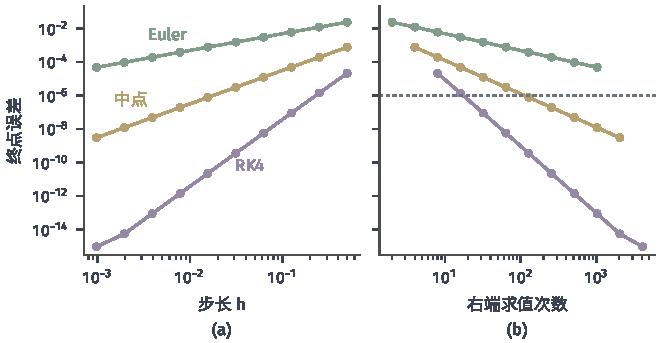
\includegraphics[width=112mm]{figures/06-differential-equations/01-ordinary-differential-equations/matplotlib/odenum-rk-convergence/figure.pdf}
 \caption{三种方法在式~\eqref{eq:odenum-running}上$t=1$处的误差。绿、黄、紫线分别是Euler、中点、RK4。(a)误差对步长；(b)误差对右端求值次数，灰色虚线是$10^{-6}$。RK4在$h$很小时误差碰到舍入水平。}
 \label{fig:odenum-rk-convergence}
\end{BookInlineFigure}

\begin{BookInlineTable}
 \centering
 \caption{式~\eqref{eq:odenum-running}上使$t=1$处误差不超过给定精度所需的右端求值次数（步数以约$3\%$递增搜索，故为近似值）。}
 \label{tab:odenum-cost}
 \begin{tabular}{rrrr}
  \toprule
  目标精度 & Euler（每步1次） & 中点（每步2次） & RK4（每步4次）\\
  \midrule
  $10^{-2}$ & 5 & 2 & 4\\
  $10^{-4}$ & $5.0\times10^{2}$ & 12 & 8\\
  $10^{-6}$ & $4.9\times10^{4}$ & $1.2\times10^{2}$ & 20\\
  $10^{-8}$ & $5.0\times10^{6}$ & $1.1\times10^{3}$ & 56\\
  \bottomrule
 \end{tabular}
\end{BookInlineTable}

表中的规律是：精度要求越高，高阶方法的优势越大；要求只有$10^{-2}$时，三者的成本差不多，RK4反而比中点方法多花一倍。这个比较只在解足够光滑时有意义，图~\ref{fig:odenum-rk4-jump}的情形下RK4多花的求值次数并不能换来四阶精度。

